\chapter{Installation}
\label{cha:Installation}

\section{Download Already Built \CGG{}}%
\label{sec:download_already_built_cinelerra_gg}

\begin{figure}[htpb]
	\centering
	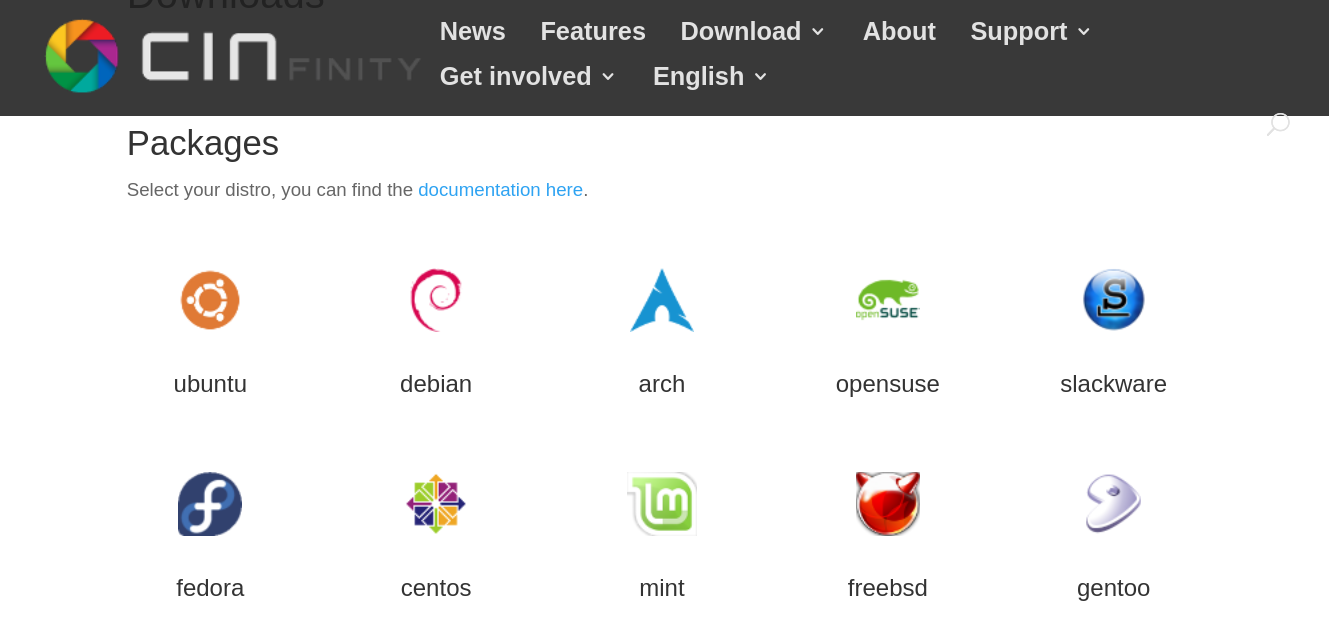
\includegraphics[width=1.0\linewidth]{download-distros.png}
	\caption{Screencast of the website Download page for installing \CGG{} for various O/S.}
	\label{fig:download-distros}
\end{figure}

If you prefer to not have to take the time to build \CGG{} Infinity
yourself, there are pre-built dynamic or static binaries for various
versions of Ubuntu, Mint, Suse, Fedora, Debian, Centos, Arch, and
Slackware linux as well as Gentoo and FreeBSD.  If you do want to build it yourself so that
you get the added benefit of the latest checked in changes, please reference
~\ref{sec:How_to_build}.
%
A Windows 10 version installation is described in~\ref{sec:ms_windows10}.  There are also 32-bit i686 Ubuntu, Debian,
and Slackware versions available.  These are updated on a fairly
regular basis as long as significant code changes have been made.
They are in subdirectories of:

\begin{list}{}{}
	\item \href{https://cinelerra-gg.org/download/tars}{https://cinelerra-gg.org/download/tars}
	\item \href{https://cinelerra-gg.org/download/pkgs}{https://cinelerra-gg.org/download/pkgs}
\end{list}

The \textbf{tars} directory contains single-user static builds for
different distros.
%
This is the recommended usage of \CGG{} because all of the files
will exist in a single directory.  Generally all of the necessary
libraries are built into the static build, but in some cases you may
have to install another library that is being called for.
%
To install the single user builds, download the designated tarball
from the \texttt{./tars} subdirectory and unpack as indicated below:

\begin{lstlisting}[style=sh]
	cd /path
	mkdir cin
	cd cin
	tar -xJf /src/path/cinelerra-5.1-*.txz  # for the *,
	# substitute your distro tarball name
\end{lstlisting}

\emph{Do not download the LEAP 10-bit version unless you specifically want to
use h265 rendering to 10-bit instead of the more standard 8-bit.} For more
information see ~\ref{sec:cinx_and_a_bit_of_confusion}.

The \textbf{pkgs} directory contains the standard packaged
application for various distros.  This will install a dynamic
system version for users who prefer to have the binaries in the
system area and for multi-user systems.
%
In addition, performing the package install checks the md5sum in
the file \texttt{md5sum.txt} to ensure the channel correctly
transmits the package.  There is a
\href{https://cinelerra-gg.org/download/README.pkgs}{README.pkgs}
file in the \texttt{download} directory with instructions so you
can \textit{cut and paste} and avoid typos; it is also shown
next.

\lstset{inputpath=extra/}
\lstinputlisting[
style=nil,
basicstyle=\footnotesize,
caption={README.pkgs}
]{README.pkgs}

\section{How to Build \CGG{} from Developer's Git Repository}%
\label{sec:How_to_build}

These are generic build instructions for building \CGG{} Infinity.
Known to work on Ubuntu, Mint, OpenSuse, Fedora, Debian, Centos,
Arch, Slackware, and Gentoo.  It has not been tested on every
single possible distro yet so you might expect to have to make
some minor changes.  Also works on a somewhat limited basis on
FreeBSD and Windows 10 with the bsd.patch for FreeBSD and the
cygwin.patch for Windows 10.

Alternatively, there are some pre-built dynamic or static binaries
which are updated on a fairly regular basis (as long as code changes
have been made) available at the link below.
\begin{center}
  \href{https://cinelerra-gg.org/download/}{https://cinelerra-gg.org/download/}
\end{center}

There are 2 kinds of builds, the default system-build and a
single-user build.  A system build has results which are installed
to the system.  The majority of the files are installed in the
standard system paths, but some customization is possible.  The
single user build allows for running completely out of a local
user directory so it doesn't affect the system.

We recommend the single-user version when possible.  It makes it
very easy to install a new version without having to delete the
older version in case you want it for backup -- once you are happy
with the new version, all you have to do is delete the entire old
directory path.  Another reason for using single-user is that if
you install a new Operating System version and if you have \CGG{}
on separate disk space that is preserved, you won't have to
reinstall \CGG{}.  It is also convenient for the purpose of having
the ability to interrupt or to see any possible error messages, if
you start the application from a terminal window command line
where you will have more control to catch problems.  All that
said, the system builds can be useful in a university lab setting
where there are possibly multiple users, or multiple versions.

There are two notable differences between standard views
of \CGG{} and this implementation for the system builds.  Both of
these can be configured during installation.  The differences make
it possible to have several different versions installed without
having them interfere with each other.

\begin{enumerate}
\item application name can be set during a build but defaults
  to: \texttt{cin}
\item the home configuration directory can also be set and
  traditionally defaults to: \texttt{\$HOME/.bcast5}
\end{enumerate}


\subsection{The system build}
\label{sec:system-build}

To do a system build, you should read the file
\texttt{README} that is at the top level after you get the source.

\begin{itemize}
\item You need about 6.0 \,GB of disk storage to operate a build and
  you need to have \textit{git} installed.

\item Obviously in order to install into the system, you must run as
  \textbf{root}.

\item The \textit{git:} step has to download many files (approx
  130\,MB) so allow time. When decompressed this will expand to
  about 530 MB.

\item Run the following commands (this takes awhile):

\begin{lstlisting}[style=sh]
# This is where you need the 6.0GB of disk space:
cd /<build_path>/
git clone --depth 1 "git://git.cinelerra-gg.org/goodguy/cinelerra.git" cinelerra5
# Change to the cloned directory:
cd cinelerra5/cinelerra-5.1
\end{lstlisting}
  NOTE: if your system has never had \CGG{} Infinity installed, you
  will have to make sure you have all of the compilers and libraries
  necessary.  So on the very first build you should run:

\begin{lstlisting}[style=sh]
./blds/bld_prepare.sh <os> # where <os> represents the
                           # Operating System of
                           # centos, fedora, suse, ubuntu, mint, debian.
./autogen.sh
./configure --prefix=/usr  # optional parameters can be added here
make 2>&1 | tee log        # make and log the build
\end{lstlisting}

  \texttt{bld\_prepare.sh} does not work for Arch Linux or Gentoo,
  so we have to install the dependencies
  manually. \texttt{README.arch} or \texttt{README.gentoo}, which
  contain the list of dependencies, can be found at:
  \begin{list}{}{}
  \item \href{https://cinelerra-gg.org/download/README.arch}{https://cinelerra-gg.org/download/README.arch}
  \item \href{https://cinelerra-gg.org/download/README.gentoo}{https://cinelerra-gg.org/download/README.gentoo}
  \end{list}

\item Check for obvious build errors:
\begin{lstlisting}[style=sh]
grep "\*\*\*.*error" -ai log
\end{lstlisting}
  If this reports errors and you need assistance or you think
  improvements can be made to the builds, email the log which is
  listed below to:
  \href{mailto:cin@lists.cinelerra-gg.org}{cin@lists.cinelerra-gg.org}
\begin{lstlisting}[style=sh]
/<build_path>/cinelerra5/cinelerra-5.1/log
\end{lstlisting}

\item If there are no build errors, finally just run:
\begin{lstlisting}[style=sh]
make install
\end{lstlisting}
Where <os> represents the Operating System supported by \CGG{}, such
as centos, fedora, suse, ubuntu, mint, debian.
The ``with-single-user'' parameter makes it so.
% Make and log build (
Check for errors before proceeding.


\item If it all worked, you are all setup. Just click on the \CGG{}
  desktop icon.
\end{itemize}


\subsection{The single-user build}
\label{sec:single-user-build}

To do a single-user build, read the file \texttt{README} that is at
the top level after you get the source.

\begin{enumerate}
\item You need at least 6\,GB of disk storage to operate a build +
  you need to have “\texttt{git}” installed.

\item Recommend you build and run as \textbf{root}, just to avoid
  permission issues initially.
\item The \textit{git} step has to download many files (approx
  130\,MB) so allow time.

\item Run the following commands (this takes awhile):
\begin{lstlisting}[style=sh]
# This is where you need the 6GB of disk space
cd /<build_path>/
git clone --depth 1 "git://git.cinelerra-gg.org/goodguy/cinelerra.git" cinelerra5
# Toplevel directory:
cd cinelerra5/cinelerra-5.1
\end{lstlisting}
\end{enumerate}

NOTE: if your system has never had \CGG{} Infinity installed, you
will have to make sure all the compilers and libraries necessary are
installed. So on the very first build you should run as
\textbf{root}:

% FIXME No novels in the listings.
\begin{lstlisting}[style=sh]
./blds/bld_prepare.sh <os>
./autogen.sh
./configure --with-single-user
make 2>&1 | tee log
make install
\end{lstlisting}
Where <os> represents the Operating System supported by \CGG{}, such
as centos, fedora, suse, ubuntu, mint, debian.
The ``with-single-user'' parameter makes it so.
% Make and log build (
Check for errors before proceeding.


Then just start the application by keying in: \texttt{./cin} in the
bin subdirectory OR add a desktop icon by using the appropriate
directory to copy the files to, run as \textbf{root}, and edit to
correct the directory path.  Below are generic directions of how to
do this.

Then just start the application by keying in: \texttt{./cin} in the
bin subdirectory OR add a desktop icon by using the appropriate
directory to copy the files to, run as \textbf{root}, and edit to
correct the directory path.  Below are generic directions of how to
do this.

\begin{lstlisting}[style=sh]
cd /cinelerra_directory_path
cp -a image/cin.{svg,xpm} /usr/share/pixmaps/
cp -a image/cin.desktop /usr/share/applications/cin.desktop
\end{lstlisting}

After you have followed the above, in the cin.desktop file, change
the \texttt{Exec=cin} line to be
\texttt{Exec=<your\_directory\_path>/bin/cin}.

The preceding directions for doing a single-user build may work
without being root on some distros except for the \texttt{bld\_prepare.sh}
and creating the desktop icon.


\subsection{Notable Options and Caveats}%
\label{sub:notable_options_and_caveats}

These procedures and the \CGG{} Infinity software have all been run
as \textbf{root} on various home laptops and desktops. This provides
the best chance to ensure all works correctly and also allows for
handling errors, other problems and potential crashes with the most
success.  Included in this section are some of the build variations
easily available for normal builds.

To see the full list of features use:

\begin{lstlisting}[style=sh]
./configure --help
\end{lstlisting}
The default build is a system build which uses:

\begin{lstlisting}[style=sh]
./configure --without-single-user
\end{lstlisting}

In the single-user build, the target directory is always
\texttt{cin}.  Because this is also the developer build, constant
names are used throughout.  However, you can rename files after the
install is complete.

If your operating system has issues with the default install to
\texttt{/usr/local}, you might have to change the location to
\texttt{/usr} for a system build.  Then you will have to use:
\begin{lstlisting}[style=sh]
./configure --prefix=/usr
\end{lstlisting}

If you wish to change the default directory for a system build you
will have to add the destination directory path on the \texttt{make
  install} line.  For example:
\begin{lstlisting}[style=sh]
make install DESTDIR=<your selected target directory path>
\end{lstlisting}

The application name can be set during installation, but defaults to
\texttt{cin} so that the GG/Infinity build can coexist with other
\CGG{} builds if necessary.  To override the default \texttt{cin}
name, use:
\begin{lstlisting}[style=sh]
./configure --with-exec-name=cinelerra
\end{lstlisting}

The home configuration directory can also be set, but default
location is traditionally \texttt{\$HOME/.bcast5}.  For example:

\begin{lstlisting}[style=sh]
./configure -with-config-dir=/myusername/.bcast5
\end{lstlisting}

NOTE: when you specify parameters to the configure program, it will
create a \texttt{make} file as a consequence.  Since in a
\texttt{make} file, the \$ is a special character, it must be
escaped so in order to represent a \$ as part of an input parameter,
it has to be stuttered.  That is, you will need \$\$ (2 dollar
signs) to represent a single dollar sign.

It may be necessary on some distros which have missing or incomplete
up-to-date libraries, to build \CGG{} without Ladspa.  To do so,
use:

\begin{lstlisting}[style=sh]
./configure --prefix=/usr --without-ladspa-build
\end{lstlisting}

Note that the with-ladspa-dir is the ladspa search path, and
exists even if the ladspa build is not selected.  This gives you
the ability to specify an alternate ladspa system path by
utilizing the \texttt{LADSPA\_PATH} environment variable (that is,
the default ladspa build is deselected).

Note for 32-bit 14.2 Slackware, Debian, Gentoo, Arch, FreeBSD,
before running the configure, you will need to set up the following:

\begin{lstlisting}[style=sh]
export ac_cv_header_xmmintrin_h=no
export FFMPEG_EXTRA_CFG=" --disable-vdpau"
\end{lstlisting}


\subsection{Notes about Building from Git in your Customized Environment}%
\label{sub:notes_about_building_from_git_in_your_customized_environment}

Getting a build to work in a custom environment is not easy.  If you
have already installed libraries which are normally in the
thirdparty build, getting them to be recognized means you have to
install the \textit{devel} version so the header files which match
the library interfaces exist.  Below is the list of thirdparty
builds, but this list may have changed over time.
% It's list of Table?

\begin{table}[htpb]
  \centering
  \caption{List of thirdparty builds}
  \label{tab:List_of_thirdparty_builds}
  \small
  \begin{tabular}{m{8em}c}
    \toprule
 	a52dec   & yes\\
 	djbfft   & yes\\
 	ffmpeg   & yes\\
 	fftw     & auto\\
 	flac     & auto\\
 	giflib   & yes\\
 	ilmbase	 & auto\\
 	lame     & auto\\
 	libavc1394&auto\\
 	libraw1394&auto\\
 	libiec61883&auto\\
    libdv     &auto\\
 	libjpeg   &auto\\
 	opus	  &auto\\
 	openjpeg  &auto\\
 	libogg    &auto\\
 	libsndfile&auto\\
 	libtheora&auto\\
 	libuuid  & yes\\
 	libvorbis&auto\\
 	mjpegtools&yes\\
 	openexr   &auto\\
    tiff      &auto\\
 	twolame   &auto\\
 	x264      &auto\\
 	x265      &auto\\
 	libvpx    &auto\\
 	lv2       &auto\\
 	sratom    &auto\\
 	serd      &auto\\
 	sord      &auto\\
 	lilv      &auto\\
 	suil      &auto\\
 	libaom    &auto\\
 	dav1d     &auto\\
    libwebp   &auto\\
 	ffnvcodec &auto\\
    \bottomrule
  \end{tabular}
\end{table}


The \textit{yes} means force build and \textit{auto} means probe and
use the system version if the build operation is not static.  To get
your customized build to work, you need to change the probe options
for the conflicting libraries from \textit{yes} to \textit{auto}, or
even rework the \texttt{configure.ac} script.  There may be several
libraries which need special treatment.

An example of a problem you might encounter with your customized
installation is with \texttt{a52dec} which has probes line
\texttt{(CHECK\_LIB/CHECK\_HEADERS)} in \texttt{configure.ac}, but
\texttt{djbfft} does not.  In this case, \texttt{djbfft} is only
built because \texttt{a52dec} is built, so if your system has
\texttt{a52dec}, set \texttt{a52dec} to auto and see if that
problem is solved by retrying the build with:
\begin{lstlisting}[style=sh]
./confgure --with-single-user -enable-a52dec=auto .
\end{lstlisting}

With persistence, you can get results, but it may take several tries
to stabilize the build.  If you need help, email the \texttt{log}
and \texttt{config.log}, which is usually sufficient to determine
why a build failed.

If you have already installed the \texttt{libfdk\_aac} development
package on your computer because you prefer this version over the
default aac, you will have to do the following to get this
alternative operational. The libfdk\_aac library is not a part of
\CGG{} by default because it is not license free.

\begin{lstlisting}[style=sh]
export FFMPEG_EXTRA_CFG=" --enable-libfdk-aac --enable-nonfree"
export EXTRA_LIBS=" -lfdk-aac"
for f in `grep -lw aac cinelerra-5.1/ffmpeg/audio/*`; do
  sed -e 's/\<aac\>/libfdk_aac/' -i $f
done
\end{lstlisting}


\subsection{Cloning the Repository for Faster Updates}%
\label{sub:cloning_the_repository_for_faster_updates}

If you want to avoid downloading the software every time an update
is available you need to create a local ``repository'' or repo.  The
repo is a directory where you first do a \texttt{git clone}.  For
the initial git clone, set up a local area for the repository
storage, referred to as \texttt{<repo\_path>}.  The \texttt{git
  clone} creates a repo named \texttt{cin5} in the
\texttt{/<repo\_path>/} directory.  This accesses about 530\,MB of
repo data, so the device has to have at least that available.  The
repo path is always a perfect clone of the main repo.


\paragraph{Setting up the initial clone}%
\label{par:setting_up_the_initial_clone}

You may want to add ``\verb|--depth 1|'' before \texttt{cin5}
because this will clone faster and is smaller, but has no history.

\begin{lstlisting}[style=sh]
cd /<repo\_path>/
git clone "git://git.cinelerra-gg.org/goodguy/cinelerra" cin5

Cloning into "cin5"...
remote: Counting objects: 20032, done.
remote: Compressing objects: 100% (11647/11647), done.
remote: Total 20032 (delta 11333), reused 16632 (delta 8189)
Receiving objects: 100% (20032/20032), 395.29 MiB | 3.26 MiB/s, done.
Resolving deltas: 100% (11333/11333), done.
Checking connectivity... done.
\end{lstlisting}


\paragraph{Update an existing repo}%
\label{par:update_an_existing_repo}
The below shows how you can get updates.

\begin{lstlisting}[style=sh]
cd /<repo home>/cin5
git pull
\end{lstlisting}


\paragraph{Useful git commands}%
\label{par:useful_git_commands}
Some other commands that are useful.

\begin{lstlisting}[style=sh]
git clone "git://git.cinelerra-gg.org/goodguy/cinelerra.git" cin5
git pull         # pull remote changes to the local version
git status       # shows changed files
git clean -i     # interactive clean, use answer 1 to "clean"
\end{lstlisting}


\subsection{How to Build from a Previous GIT Version}%
\label{sub:how_to_build_from_a_previous_git_version}

If you have a problem with the current GIT version, you can revert
to a previous working version easily.  The commands to use will be
similar to these next lines which are then explained in more detail.
\strut
 
\begin{lstlisting}[style=sh]
cd /<path>/cin5  # substitute your repo path name for cin5
git log		 # shows a list of versions depending on history depth specification
git checkout <version> # choose a version number as listed
\end{lstlisting}

The \texttt{git log} command produces a log file with hash values
for commit keys to the level specifed if the the depth paramter
was specified. 
The hash ids are the commit names to use when you
use git checkout. Next is displayed sample output:

\begin{lstlisting}[style=nil]
delete stray line in last checkin

commit 4a90ef3ae46465c0634f81916b79e279e4bd9961
Author: Good Guy <good1.2guy@gmail.com>
Date: Thu Feb 22 14:56:45 2018 -0700

nested clips, big rework and cleanup, sams new icons,
leaks and tweaks

commit f87479bd556ea7db4afdd02297fc00977412b873
Author: Good Guy <good1.2guy@gmail.com>
Date: Sat Feb 17 18:09:22 2018 -0700
\end{lstlisting}

For the \texttt{git checkout <version>}, you would then keyin the
line below for the following results:

\begin{lstlisting}[style=nil]
git checkout f87479bd556ea7db4afdd02297fc00977412b873

Note: checking out 'f87479bd556ea7db4afdd02297fc00977412b873'.

You are in 'detached HEAD' state. You can look around, make
experimental changes and commit them, and you can discard any
commits you make in this state without impacting any branches by
performing another checkout.

If you want to create a new branch to retain commits you create,
you may do so (now or later) by using -b with the checkout command
again. Example:

git checkout -b <new-branch-name>

HEAD is now at f87479bd... more file size icon updates,
and more to followend
\end{lstlisting}

Later to get the repo back to current, use:
\begin{lstlisting}[style=sh]
git checkout master
\end{lstlisting}


\subsection{Debuggable Single User Build}%
\label{sub:debuggable_single_user_build}

To build from source with full debugging symbols, first build a full
static (non\_debug) build as follows but instead of using
\texttt{/tmp} substitute your permanent disk path if you want to
keep it.

\begin{lstlisting}[style=sh]
cd /<repo_path>/
git clone --depth 1 "git://git.cinelerra-gg.org/goodguy/cinelerra.git" cinelerra5 
cp -a /<repo_path>/cinelerra-5.1 /tmp/
cd /tmp/cinelerra-5.1
./bld.sh
\end{lstlisting}

Then, to run as a developer in the debugger:

\begin{lstlisting}[style=sh]
CFLAGS="-O2 -ggdb" make -j8 rebuild_all
cd cinelerra
gdb ./ci
\end{lstlisting}


\subsection{Unbundled Builds}%
\label{sub:unbundled_builds}

There are some generic build scripts included in the \CGG{} GIT
repository for users who want to do unbundled builds with ffmpeg
already available on their system.  This has been tested on Arch,
Ubuntu 18, FreeBSD, Windows10 and Leap 15 (rpm) at the time this
was documented.
%
The names of the build scripts are: \texttt{arch.bld},
\texttt{bsd.bld}, \texttt{deb.bld}, \texttt{rpm.bld}, and
\texttt{cygwin.bld}.  These scripts are in the \texttt{blds}
subdirectory.  The \texttt{bsd.bld} should be used with the
\texttt{bsd.patch} file in that same directory.  The
\texttt{cygwin.bld} should be used with the \texttt{cygwin.patch}
file in that same directory.

The reason that Cin Infinity traditionally uses its own thirdparty builds
(bundled builds) is because there are a lot of different distros
with varying levels of ffmpeg and other needed thirdparty
libraries.  However, some users prefer using their current system
baseline without another/different copy of ffmpeg.
%
With different levels of the user’s libraries, uncertainty,
potential instability, and unknown issues may come up while
running \CGG{} and this will make it, for all practical purposes,
impossible to diagnose and debug problems or crashes.
%
There may be no help in these cases.  You are encouraged to report
any errors which potentially originate from Cin Infinity, but if
the data indicates alternate library sources, please report the
problems to the appropriate maintainers.

With the unbundled builds, some features may not be available and
no attempt to comment them out has been made.  So if you use a
pulldown, or pick a render option, or choose something that is not
available, it just will not work.  For example, unless special
options were set up by you, the LV2 audio plugins will not be
available.  Nor will the codec libzmpeg, the file codec ac3, or
DVD creation.  The old school file classes will all work, but some
of the formats that come with ffmpeg may not because of the way
that ffmpeg was installed on your operating system.  That is
because the \CGG{} included ffmpeg is a known static build and is
usually the latest stable/released version.  For example, in the
current case of Leap 15, libx264 and libx265 are not built in and
this can be debilitating; you can always run \texttt{ffmpeg
  -formats} and \texttt{ffmpeg -codecs} to see what is available
on your system.

\section{Windows 10 with Cygwin for \CGG{} Limited}%
\label{sec:ms_windows10}

To run \CGG{} on a Windows 10 computer, you will need to have
Cygwin installed on your system, along with the \CGG{} static tar
and a patched library: libxbc.  This setup has been tested with
Windows 10, version 1909, on an HP EliteBook 820 at 2.3 GHz.

This limited version provides \textit{core} functionality at this
time with the standard Windows FFmpeg executable, meaning that
specific modifications in FFmpeg needed for \CGG{} are not
available.  Limited capabilities include only a few render output
formats available - for example \textit{mov}, \textit{qt} as
\textit{mjpeg}, and \textit{mpeg} for videos and \textit{avi} and
\textit{qt} as \textit{s16le} for audio, but not \textit{mkv} or
\textit{mp4}.  This is due to the fact that several codec and
utility libraries are not currently compiled to work with Windows.

\subsection*{Installing Cygwin}
\label{sec:installing_cygwin}

Cygwin is an environment that runs natively on Windows which
allows Unix programs to be compiled and run on Windows.  With
cygwin installed on your Windows 10 computer, you will be able to
run \CGG{}.  Before installing cygwin, you need to be warned that
the Avast anti-virus software kills files necessary for cygwin
installation and execution, so you will have to remove it and use
alternative anti-virus software (the standard default already
included with Windows 10 is Defender). Below are the steps for
installation:

\begin{enumerate}
\item Download cygwin for your 64-bit computer at:
  \href{https://www.cygwin.com/}{https://www.cygwin.com/}

\item Generally just take the defaults as they show up, but the
  next steps show what comes up.

\item When a warning window pops up, click \textit{Yes}.

\item Click \textit{Next}.

\item Choose \textit{Install from Internet} option and then click
  \textit{Next}.

\item Choose your desired directory by clicking on Browse
  button. Choose \textit{All Users (Recommended)} and then click
  \textit{Next}.

\item Choose the local package directory where you would like your
  installation files to be placed. Click \textit{Next}.

\item Choose \textit{Direct Connection} if you are using Internet
  with plug and play device. Click \textit{Next}.

\item Choose any download site preferably
  ``cygwin.mirror.constant.com'' and then click \textit{Next}.

\item For list of things to install, leave all set to
  \textit{Default} except these to \textit{Install} instead:

  \begin{tabular}{ll}
    base& devel\\
    gnome& graphics\\
    system& video\\
    X11
  \end{tabular}

  This install takes a long time; approximately 2 hours on an
  EliteBook and requires approximately 20GB storage.

\item Finally you will want to have the icons on your desktop
  (already default) and then click \textit{Finish}.
\end{enumerate}

Then to install the \CGG{} tar files, you will need to start a
cygwin console terminal from the startup menu as shown here:
\texttt{Start $\rightarrow$ Cygwin $\rightarrow$ Cygwin64}
Terminal

\subsection*{Installing \CGG{}}
\label{sec:installing_cinelerra}

\begin{enumerate}
\item Download the tar file
  \href{https://cinelerra-gg.org/download/testing/libxcb-bld.tar.bz2}{libxcb-bld.tar.bz2}.

\item Install libxbc from the tar file -- installs into
  \texttt{/usr/local} and requires approximately 21MB storage.
\begin{lstlisting}[style=sh]
tar -C /usr/local -xJf /path/libxcb-bld.tar.bz2
\end{lstlisting}
  The libxcb path repairs an error (XIOError), which stops
  Cinelerra.

\item Download the tar file
  \href{https://cinelerra-gg.org/download/testing/cygcin-bld.tar.bz2}{cygcin-bld.tar.bz2}.

\item Install cygcin from the tar file - this installs into home
  directory.  Note this is cygcin \emph{not} cygwin. You must change the
  \texttt{path} below to the name of the path where you downloaded
  the tar file.
\begin{lstlisting}[style=sh]
cd
tar -xJf /path/cygcin-bld.tar.bz2
\end{lstlisting}
\end{enumerate}

This creates \texttt{\~{}/cygcin}, a user build installation of
\CGG{} and requires approximately 400MB storage.

\paragraph{Running \CGG{}:}
You will need to start a cygwin desktop from the startup menu:
\begin{enumerate}
\item \texttt{Start$\rightarrow$ Cygwin-X $\rightarrow$ Openbox}

  You should start a console controlling terminal so that you can
  see program logging.

\item \texttt{Start$\rightarrow$ Cygwin $\rightarrow$ Cygwin64} Terminal

  This opens a separate window that can survive a cygwin hang and
  bugs. Without these logs, it is much more difficult to use.

\item Type into that console controlling window, the following:
\begin{lstlisting}[style=sh]
export DISPLAY=:0.0
\end{lstlisting}

\item Change directories to where \CGG{} is installed:
\begin{lstlisting}[style=sh]
cd /path/cygcin    (NOT cygwin)
\end{lstlisting}

\item Finally keyin:
\begin{lstlisting}[style=sh]
./cin
\end{lstlisting}
  which starts up your 4 \CGG{} windows.
\end{enumerate}

The most noticeable difference from the Linux versions is that
\CGG{} seems to run very slowly on Windows 10. You must be very
tolerant and patient to see this work.  It can however exhibit
astonishing speed when encoding.  \CGG{} has to be downgraded
significantly due to lack of supported interfaces, codecs (for
example h264/h265), and utilities.  The only graphics driver is
X11 and the only sound driver is pulseaudio.  Almost all
configurable omissions are applied to this build.

\paragraph{\CGG{} build on cygwin from source code:}

\begin{enumerate}
\item Download and install ffmpeg into /usr/local :

  download ffmpeg (currently 4.2.2)
\begin{lstlisting}[style=sh]
cd /tmp
tar -xJf /path/ffmpeg-4.2.2.tar.bz2
cd ffmpeg-4.2.2
./configure
make -j
make install
\end{lstlisting}

\item Download and install a patched libxcb:
\begin{lstlisting}[style=sh]
cd /tmp
rm -rf libxcb-1.13/
tar -xf /path/libxcb-1.13.tar.bz2
cd libxcb-1.13/
patch -p1 < /path/cinelerra-5.1/thirdparty/src/libxcb.patch1
   patching file configure.ac
   patching file src/xcb_in.c
./autogen.sh
./configure
make -j
make install
\end{lstlisting}
\item Download cinelerra-gg:
\begin{lstlisting}[style=sh]
cd /build_path/
git clone "git://git.cinelerra-gg.org/goodguy/cinelerra.git"
cd cinelerra-gg/cinelerra-5.1
\end{lstlisting}
\item Apply cygwin patch:
\begin{lstlisting}[style=sh]
patch -p2 < blds/cygwin.patch
\end{lstlisting}
\item Run the build with:
\begin{lstlisting}[style=sh]
./blds/cygwin.bld
\end{lstlisting}
\end{enumerate}

This produces a directory: /build\_path/cinelerra-gg/cinelerra-5.1/bin
which is used to create the cygcin archive.

Currently, the targets are not stripped and can be run from gdb.
There is only very limited signal handler dmp file support.
Running gdb from inside a desktop resident console (not a cygwin64
window) will hang cygwin (and cin) when it hits a breakpoint.  You
must run from an external console window to avoid this issue.


\section{Distribution Systems with \CGG{} Included}%
\label{sec:distribution_systems_with_cinelerra_included}

There are also some special complete distribution systems
available that include \CGG{} for audio and video production
capabilities.

\subsection{AV Linux}
\label{sec:AV_Linux}

\textbf{AV Linux} is a downloadable/installable shared snapshot
ISO image based on Debian.  It provides the user an easy method to
get an Audio and Video production workstation without the hassle
of trying to find and install all of the usual components
themselves.  Of course, it includes \CGG{}!
%
Click here for the
\href{http://www.bandshed.net/avlinux/}{homepage of AV Linux}.

\subsection{Bodhi Linux Media}
\label{sec:Bodhi_Linux}

\textbf{Bodhi Linux Media} is a free and open source distribution that
comes with a curated list of open source software for digital
artists who work with audio, video, includes \CGG{}, games,
graphics, animations, physical computing, etc.
%
Click here for the
\href{https://gitlab.com/giuseppetorre/bodhilinuxmedia}{homepage of Bodhi Linux}.

\subsection{Elive}
\label{sec:elive}

\textbf{Elive}, or Enlightenment live CD, is a non-commercial, cost-free operating system based on Debian, for the daily use and it can be used both as live CD or Installed system. Elive uses a customized Enlightenment desktop. It is fast, user-friendly and feature-rich and \CGG{} is included in the 64 bit version.

Click \href{https://www.elivecd.org/}{Elive} for more information.

\section{Cinx and a “Bit” of Confusion}%
\label{sec:cinx_and_a_bit_of_confusion}

Cinx is the exact same program as Cin.  The X (x) represents the
roman numeral 10 for 10-bit as opposed to 8-bit standard.  The
third-party library used for x265 must be specially compiled with
\texttt{--bit-depth=10} in order to produce 10-bit rendered
output.  A cinx version can be built for most other distros if 
rendering at 10-bit is desirable instead of 8-bit.
%
This build will not be able to output 8-bit depth which means you
have to retain the Cin version also.
%
Whatever build ffmpeg is linked to will determine what bit depth
it can output.  This is why there have to be separate builds.  If
you install both packages, Cin and CinX, you may get \textit{file
  conflicts of same file name} --- just continue.

Keep in mind that the regular 8-bit version works on 8-bit bytes
--- the standard word size for computers, but the 10-bit version
has to use 2 words to contain all 10 bits so you can expect
rendering to be as much as twice as slow.
%
There is also a 12-bit version for consideration but currently the
results are simply the same as 10-bit with padding to make 12-bit
so it is of no value.


%%% Local Variables:
%%% mode: latex
%%% TeX-master: "../CinelerraGG_Manual"
%%% End:
